\documentclass[landscape,a0paper,fontscale=0.292]{baposter}

\usepackage[vlined]{algorithm2e}
\usepackage{times}
\usepackage{calc}
\usepackage{url}
\usepackage{graphicx}
\usepackage{amsmath}
\usepackage{amssymb}
\usepackage{relsize}
\usepackage{multirow}
\usepackage{booktabs}
\usepackage{natbib}
\usepackage{wrapfig}

\usepackage{graphicx}
\usepackage{multicol}
\usepackage[T1]{fontenc}
\usepackage{ae}
\usepackage{enumitem}

\usepackage{colortbl}
\usepackage{xcolor}
\graphicspath{{images/}{imgs/}}

\bibliographystyle{plain}


\setlist[itemize]{leftmargin=*,nosep}
 \setlength{\columnsep}{0.7em}
 \setlength{\columnseprule}{0mm}


\renewcommand{\bibsection}{}
\newlength{\leftimgwidth}

% %%%%%%%%%%%%%%%%%%%%%%%%%%%%%%%%%%%%%%%%%%%%%%%%%%%%%%%%%%%%%%%%%%%%%%%%%%%%%%%%
% % Save space in lists. Use this after the opening of the list
% %%%%%%%%%%%%%%%%%%%%%%%%%%%%%%%%%%%%%%%%%%%%%%%%%%%%%%%%%%%%%%%%%%%%%%%%%%%%%%%%
 \newcommand{\compresslist}{%
 \setlength{\itemsep}{0pt}%
 \setlength{\parskip}{0pt}%
 \setlength{\parsep}{0pt}%
 }
\renewcommand{\rmdefault}{ptm} % Arial
\renewcommand{\sfdefault}{ptm} % Arial

%%%%%%%%%%%%%%%%%%%%%%%%%%%%%%%%%%%%%%%%%%%%%%%%%%%%%%%%%%%%%%%%%%%%%%%%%%%%%
%% Begin of Document
%%%%%%%%%%%%%%%%%%%%%%%%%%%%%%%%%%%%%%%%%%%%%%%%%%%%%%%%%%%%%%%%%%%%%%%%%%%%%
\begin{document}
%%%%%%%%%%%%%%%%%%%%%%%%%%%%%%%%%%%%%%%%%%%%%%%%%%%%%%%%%%%%%%%%%%%%%%%%%%%%%
%% Here starts the poster
%%---------------------------------------------------------------------------
%% Format it to your taste with the options
%%%%%%%%%%%%%%%%%%%%%%%%%%%%%%%%%%%%%%%%%%%%%%%%%%%%%%%%%%%%%%%%%%%%%%%%%%%%%
\begin{poster}{
 % Show grid to help with alignment
 grid=false,
 columns=5,
 % Column spacing
 colspacing=1em,
 % Color style
 headerColorOne=white,
 borderColor=cyan!30!white!90!black,
 % Format of textbox
 textborder=none,
 % Format of text header
 headerborder=none,
 headershape=rectangle,
 boxshade=none,
 headershade=plain,
 background=plain,
 bgColorOne=white,
 headerheight=0.10\textheight}
 % Eye Catcher
 {
      
\includegraphics[width=0.15\linewidth]{tables/icml_logo.png}
 }
 % Title
 {\huge\bf On Out-of-distribution Detection with Energy-based Models}
 % Authors
 {\vspace{0.3em} Sven Elflein, Bertrand Charpentier, Daniel Z\"ugner, Stephan G\"unnemann \\
 Technical University of Munich}
 %{\texttt{\{gychen, khan, kykwong\}@cs.hku.hk}}}
 % University logo
 {
      
\includegraphics[width=0.08\linewidth]{Universitaet_Logo_RGB.pdf}
      \makebox[0.04\textwidth]{} 
 }

%%%%%%%%%%%%%%%%%%%%%%%%%%%%%%%%%%%%%%%%%%%%%%%%%%%%%%%%%%%%%%%%%%%%%%%%%%%%%%
%%% Now define the boxes that make up the poster
%%%---------------------------------------------------------------------------
%%% Each box has a name and can be placed absolutely or relatively.
%%% The only inconvenience is that you can only specify a relative position 
%%% towards an already declared box. So if you have a box attached to the 
%%% bottom, one to the top and a third one which should be inbetween, you 
%%% have to specify the top and bottom boxes before you specify the middle 
%%% box.
%%%%%%%%%%%%%%%%%%%%%%%%%%%%%%%%%%%%%%%%%%%%%%%%%%%%%%%%%%%%%%%%%%%%%%%%%%%%%%

%%%%%%%%%%%%%%%%%%%%%%%%%%%%%%%%%%%%%%%%%%%%%%%%%%%%%%%%%%%%%%%%%%%%%%%%%%%%%%
\headerbox{\bf\color{blue} Problem Definition \& Contribution}{name=contribution,column=0,row=0,span=2}{
    \textbf{\color{blue}Goal:} Investigate superior OOD detection performance of EBMs vs.\ other generative models.

    \textbf{\color{blue}Motivation:}
    \begin{itemize}
        \item Recent research on density estimation focuses on exact likelihood methods.
        \item Findings of superior OOD detection performance of EBMs without analysis.
    \end{itemize} 
    \textbf{\color{blue}Key Contributions:}
    \begin{itemize}
        \item Find that EBMs do not strictly outperform Normalizing Flows across multiple training methods.
        \item Identify that learning semantic features induced by supervision improves OOD detection in recent discriminative EBMs.
        \item Show that one can use architectural modifications to improve OOD detection with EBMs.
    \end{itemize}  
}

%%%%%%%%%%%%%%%%%%%%%%%%%%%%%%%%%%%%%%%%%%%%%%%%%%%%%%%%%%%%%%%%%%%%%%%%%%%%%

%%%%%%%%%%%%%%%%%%%%%%%%%%%%%%%%%%%%%%%%%%%%%%%%%%%%%%%%%%%%%%%%%%%%%%%%%%%%%
\headerbox{\bf\color{blue} Experiments \& Results}{name=results,column=2,row=0,span=3}{
    \begin{minipage}[t]{0.48\linewidth}
    \textbf{\color{blue}Differentiation of natural and non-natural dataset.}\\
    \underline{\textit{Natural OOD}}: Requires learning semantic features to differentiate, e.g., images of classes not in training set. \\
    \underline{\textit{Non-natural OOD}}: Requires detection farther from the training data manifold, e.g., noise, OODomain

    \vspace{1em}

    \textbf{\color{blue}Are EBMs better than Normalizing Flows?}\\
    EBMs do not consistently outperform Normalizing Flows across different training methods (Improvements: CD \(11.9\% \), VERA \(4.3\% \), SSM \(-4.3\% \))

    \vspace{1em}

    \textbf{\color{blue}Does supervision improve OOD detection?}
    \begin{center}
        \resizebox{.5\textwidth}{!}{
            \begin{tabular}{llrr}
\toprule
 Model    &ID dataset &  Natural &  Non-natural \\
\midrule
\multirow{4}{*}{CD} & CIFAR-10 &   -10.82 &      -9.11 \\
     & FMNIST &    47.17 &       3.24 \\
     & Segment &     1.85 &       0.89 \\
     & Sensorless &    29.72 &      -0.02 \\
\midrule
\multirow{4}{*}{SSM} & CIFAR-10 &     7.33 &     -27.94 \\
     & FMNIST &    50.61 &     -20.26 \\
     & Segment &    25.89 &     -21.94 \\
     & Sensorless &    22.13 &     -40.73 \\
\midrule
\multirow{4}{*}{VERA} & CIFAR-10 &    -1.16 &      -3.00 \\
     & FMNIST &    33.66 &     -15.53 \\
     & Segment &     4.98 &      -0.57 \\
     & Sensorless &    97.93 &       0.07 \\
\bottomrule
\end{tabular}

        }
    \end{center}
    \begin{itemize}
        \item Leveraging supervision with JEMs improves some results significantly on \textit{natural} OOD datasets
        \item Results do not improve or even degrade on \textit{non-natural} OOD datasets
        \item Investigation shows: Weighting parameter of cross-entropy loss \(\gamma \) affects the density estimates far from training data \\
        \(\rightarrow \) \textit{Non-natural} data becomes harder to detect
    \end{itemize}
    \begin{center}
        \resizebox{0.5\textwidth}{!}{
            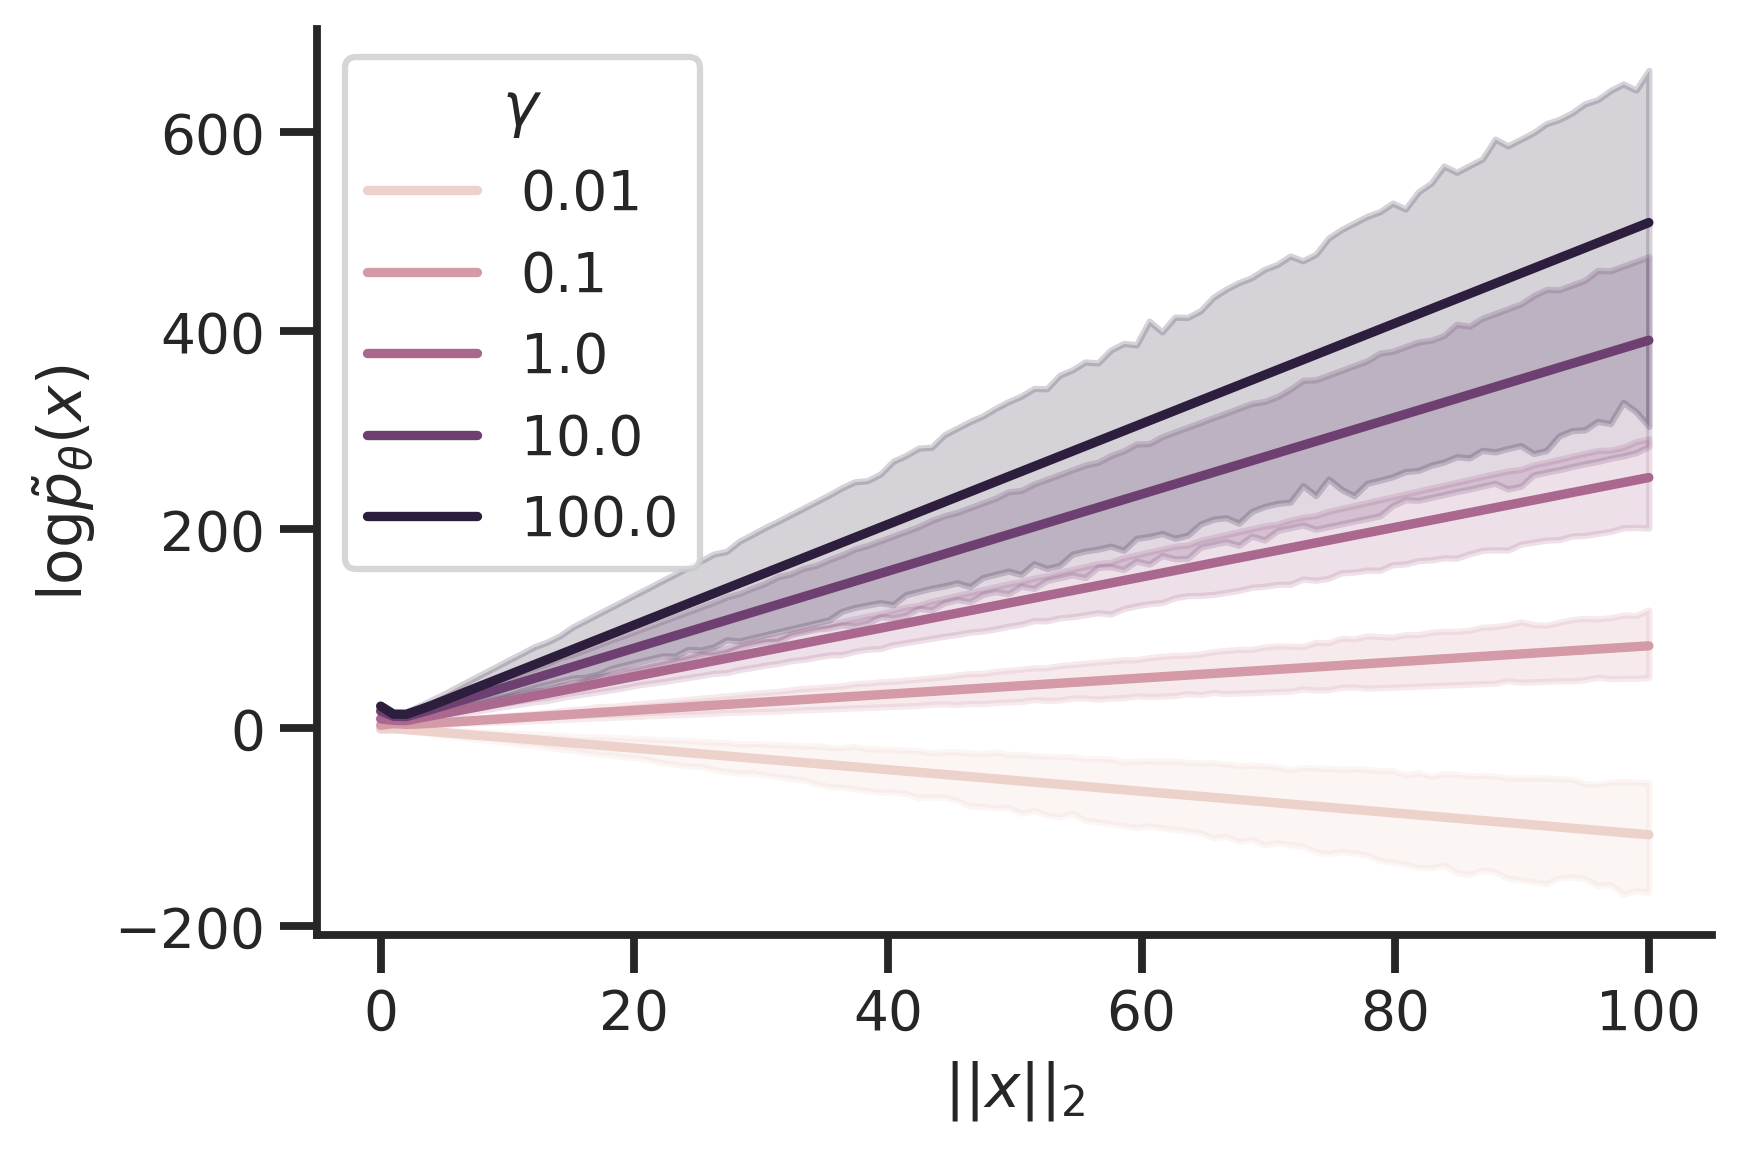
\includegraphics[width=\linewidth]{tables/clf_weight_density_from_training.png}
        }
    \end{center}
    \end{minipage}%
    \hfill
    \begin{minipage}[t]{.48\linewidth}
        \textbf{\small \color{blue}Sidestepping tuning of \(\boldsymbol{\gamma} \)}
        \begin{center}
        \resizebox{0.5\textwidth}{!}{
        \begin{tabular}{llrr}
\toprule
 Model    & ID dataset &  Natural & Non-natural \\
\midrule
\multirow{2}{*}{CD} & CIFAR-10 &    48.60 &       3.37 \\
     & FMNIST &    95.79 &     -13.52 \\
\midrule
\multirow{2}{*}{SSM} & CIFAR-10 &    53.84 &      -2.31 \\
     & FMNIST &    58.40 &      59.59 \\
\midrule
\multirow{2}{*}{VERA} & CIFAR-10 &    50.16 &      16.97 \\
     & FMNIST &    15.12 &       1.80 \\
\bottomrule
\end{tabular}

        }
        \end{center}
        \begin{itemize}
            \item Introduce supervision by training on embeddings obtained from classification model
            \item OOD detection significantly improves on \textit{natural} and in cases on \textit{non-natural} datasets
            \item Shows that vanilla EBMs struggle to extract high-level, semantic features
        \end{itemize}

        \vspace{1em}

        \textbf{\color{blue}Can we encourage semantic features?}
        \begin{center}
        \resizebox{0.5\textwidth}{!}{
        \begin{tabular}{llrr}
\toprule
 Model    & ID dataset &  Natural &  Non-natural \\
\midrule
\multirow{2}{*}{CD} & CIFAR-10 &    20.18 &        20.38 \\
     & FMNIST &    67.95 &        10.88 \\
\midrule
\multirow{2}{*}{SSM} & CIFAR-10 &    14.76 &        33.34 \\
     & FMNIST &     1.75 &        -5.92 \\
\midrule
\multirow{2}{*}{VERA} & CIFAR-10 &    19.66 &        33.22 \\
     & FMNIST &    26.84 &        32.94 \\
\bottomrule
\end{tabular}

        }
        \end{center}
        \begin{itemize}
            \item Introduce bottlenecks through \(1 \times 1\) convolutions
            \item OOD detection improves consistently upon the baseline EBMs by learning higher-level features
            \item The difference in density assigned for low-level features to images increases significantly
        \end{itemize}
        \vspace{2mm}
        \begin{minipage}[b]{0.5\linewidth}
            \begin{center}
            \resizebox{\textwidth}{!}{
                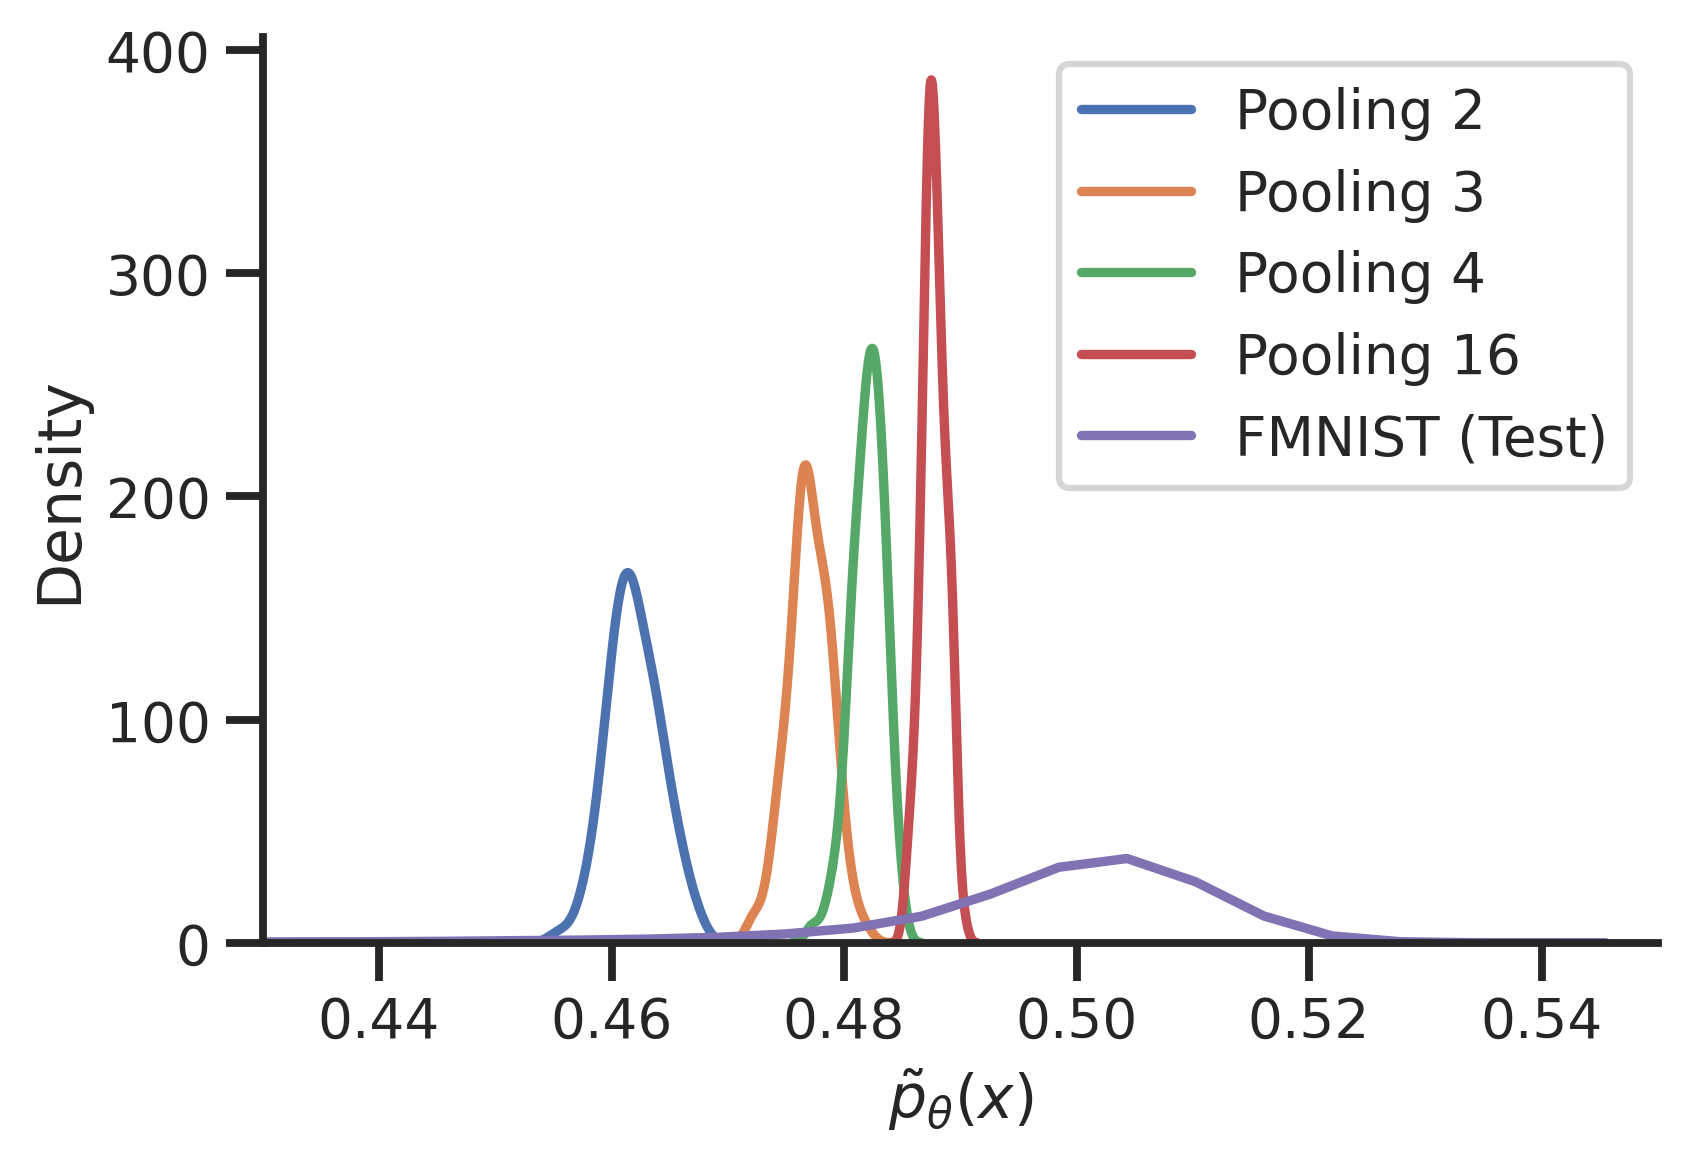
\includegraphics[width=\linewidth]{tables/no_bottleneck_pooling_density_histogram.png}
            }
            No Bottleneck.
            \end{center}
        \end{minipage}%
        \hfill
        \begin{minipage}[b]{0.5\linewidth}
            \begin{center}
            \resizebox{\textwidth}{!}{
                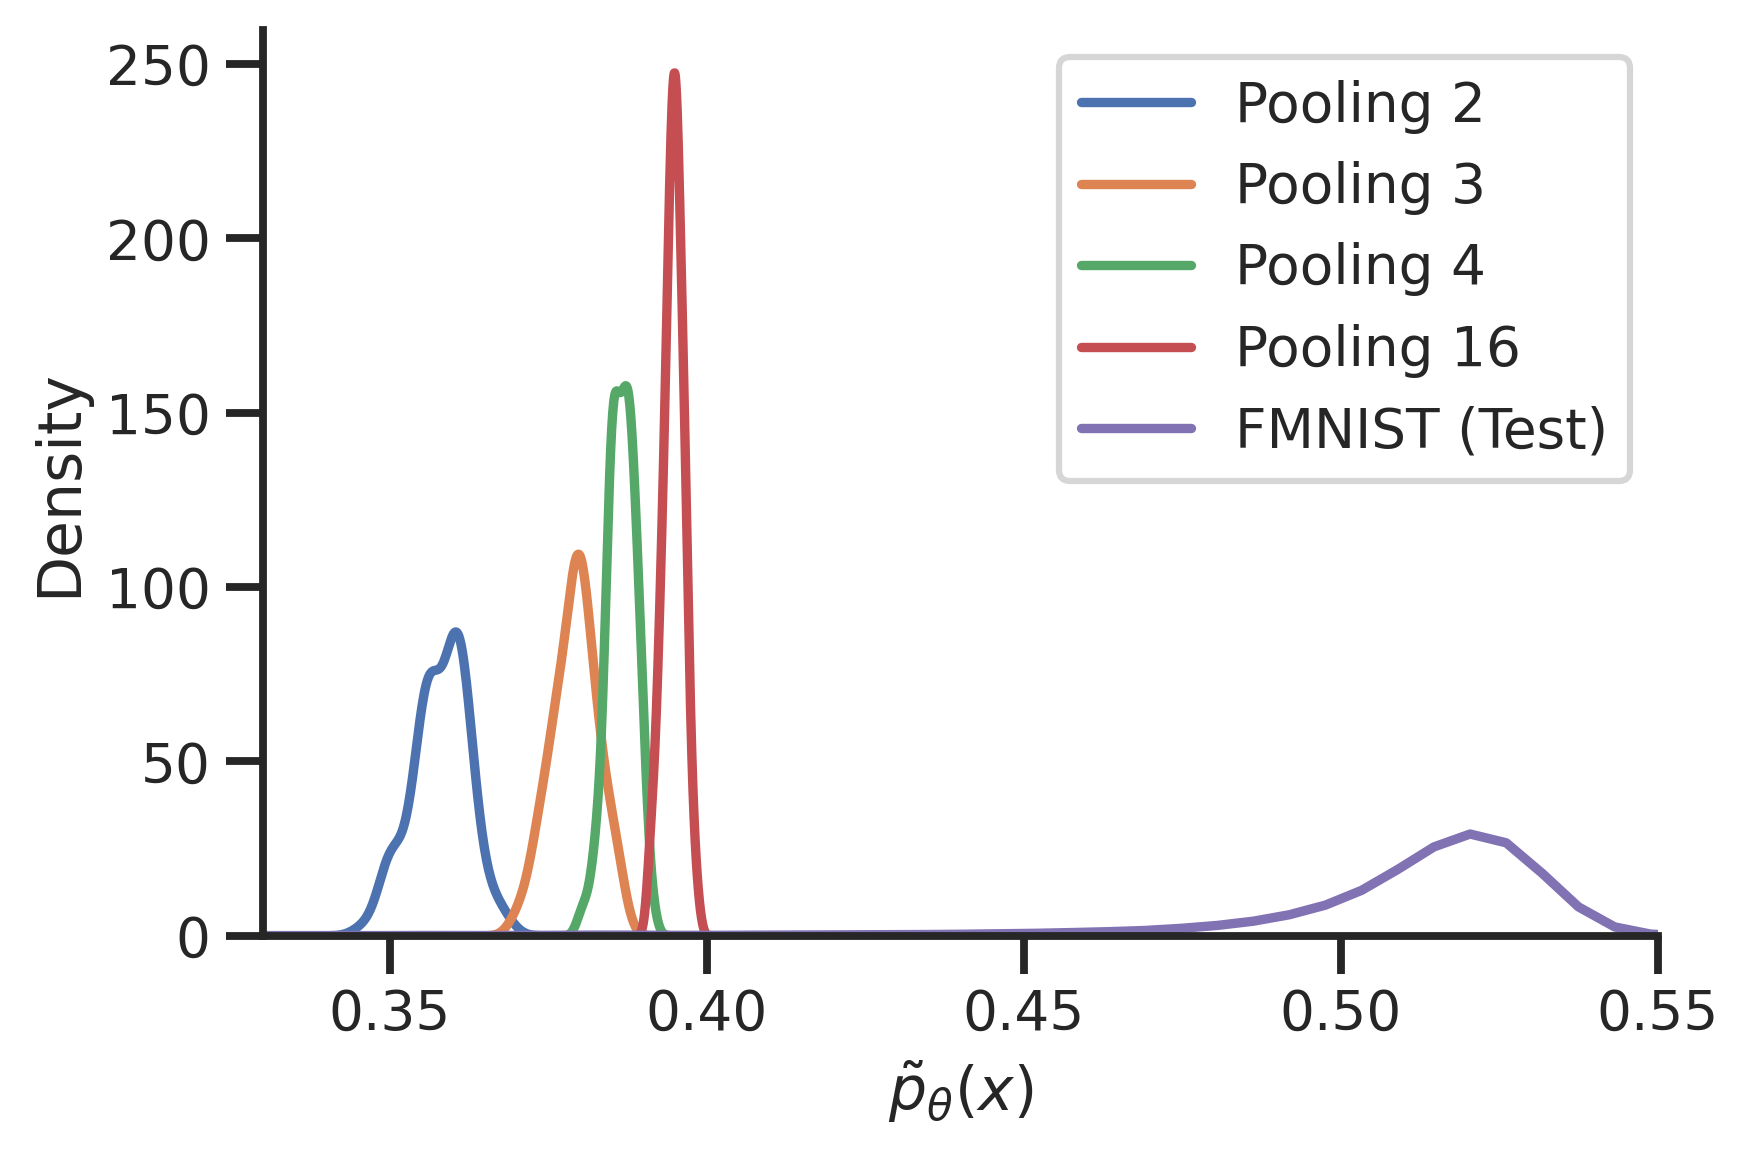
\includegraphics[width=\linewidth]{tables/bottleneck_pooling_density_histogram.png}
            }
            With Bottleneck.
            \end{center}
        \end{minipage}
    \end{minipage}%
    \vspace{-1.5em}
}

%%%%%%%%%%%%%%%%%%%%%%%%%%%%%%%%%%%%%%%%%%%%%%%%%%%%%%%%%%%%%%%%%%%%%%%%%%%%%
\headerbox{\bf\color{blue} Method}{name=abstract,column=0,below=contribution,span=2}{
    \begin{minipage}[t]{0.48\linewidth}
        \textbf{Energy-based model (EBM).}
        Energy-function \( E_\theta \) defines a density over the data \(x\) as

        \begin{equation}
            \label{eq:ebm}
            \smash{p_\theta(x) = \frac{\exp(-E_\theta(x))}{Z(\theta)}}
        \end{equation}

        where \(\smash{Z(\theta) = \int \exp(-E_\theta(x)) dx}\).% is the normalizing constant and \(\theta \) are learnable parameters. 
        % In particular, \( E_\theta \) can be any function \( E: \mathbb{R}^D \mapsto \mathbb{R} \) placing no restrictions on the model compared to Normalizing Flows. \\
        %
        \\
        \textbf{Joint Energy model (JEM)~\cite{grathwohlYourClassifierSecretly2020}.}
        Given a classifier \( f : \mathbb{R}^D \mapsto \mathbb{R}^C \) assigning logits for \(C\) classes for a datapoint \(x \in \mathbb{R}^D\)

        \begin{equation}
            \label{eq:jem_p_y_given_x}
            p_\theta(y \mid{} x) = \frac{\exp (f_\theta(x)[y])}{\sum_{y^\prime{}}\exp(f_\theta(x)[y^\prime{}])}
        \end{equation}

        where \( f_\theta(x)[y] \) denotes the \(y \)-th logit.
        %
        The logits \( f_\theta(x)[y] \) can be interpret as unnormalized probabilities of the joint distribution \(p_\theta(x, y) \)
        %
        % \begin{equation}
        %     p_\theta(x, y) = \frac{\exp(f(x)[y])}{Z_\theta}
        % \end{equation}
        which yields the marginal distribution over \(x\) as

        \begin{equation}
            \label{eq:jem_p_x}
            p_\theta(x) = \sum_y p_\theta (x, y) = \sum_y \frac{\exp(f(x)[y])}{Z(\theta)}
        \end{equation}
        \textbf{Training.}
        We follow~\cite{grathwohlYourClassifierSecretly2020} and optimize the factorization 
        %
        \begin{equation}
            \log p_\theta(x, y) =  \log p_\theta(x) + \log p_\theta(y \mid x)
        \end{equation}
        %
        using~\ref{eq:jem_p_y_given_x} and~\ref{eq:jem_p_x}. In particular, we use a Cross Entropy objective to optimize \(\smash{p_\theta(y \mid x)}\) weighted with hyperparameter \(\gamma \). \\
        %
    \end{minipage}
    \hfill
    \begin{minipage}[t]{0.48\linewidth}
        For optimizing \(p_\theta(x)\), we consider different approaches which have shown to scale to high-dimensional data. \\
        %
        \textbf{Sliced score matching (SSM)~\cite{songSlicedScoreMatching2019}.}
        Efficient update formula based on random projection
        
        \begin{equation}
            \mathbb{E}_{p_v} \mathbb{E}_{p(x)} \left[v^T \nabla_x s_\theta(x)v + \frac{1}{2} \lVert s_\theta(x) \rVert^2_2 \right]
        \end{equation}

        where \(v \sim p_v\) is a simple distribution of random vectors. \\
        %
        \textbf{Contrastive divergence (CD)~\cite{hintonTrainingProductsExperts2002}.}
        Approximation of the gradient of the maximum likelihood objective by
        %
        \begin{equation}
        \label{eq:cd}
            \nabla_\theta p_\theta(x) = \mathbb{E}_{p_\theta(x^\prime)} \left[ \nabla_\theta E_\theta(x^\prime) \right] - \nabla_\theta E_\theta(x)
        \end{equation}
        %
        \textbf{VERA~\cite{grathwohlNoMCMCMe2020}.}
        Learn the parameters \(\phi \) of a auxiliary distribution \(q_\phi \) as the optimum of
        %
        \begin{equation}
            \log Z(\theta) = \max_{q_\phi} \mathbb{E}_{q_\phi(x)} \left[ f_\theta(x) \right] + H(q_\phi)
        \end{equation}
        %
        which can be plugged into~\ref{eq:ebm} to obtain an alternative method for training EBMs with a variational approximation to estimate the entropy term \(H_{q_\phi}\).\\

        \textbf{OOD Detection.}\\ 
        For OOD detection, we compute the density \(p_\theta(x)\) at the considered datapoint \(x\). We treat ID data as class 1 and OOD data as class 0 and compute AUC-PR.
    \end{minipage}
}

\headerbox{\bf{\color{blue} References}}{name=references,column=2,below=results,span=3}{
    \footnotesize{
    \bibliography{paper}
    }
}


\end{poster}
\end{document}
